\levelstay{Coupling}

\leveldown{Capacitive coupling}

\begin{figure}
\begin{centering}
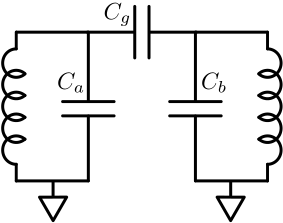
\includegraphics[width=6cm]{coupled_circuits_capacitive.pdf}
\par\end{centering}
\caption{Two circuits coupled through a capacitor $C_g$.}
\label{Fig:coupledCircuits_capacitive}
\end{figure}

The circuit shown in Fig.\,\ref{Fig:coupledCircuits_capacitive} has the Lagrangian
\begin{align}
  \mathcal{L}
  =& \frac{1}{2}C_a\dot{\Phi}_a^2 + \frac{1}{2}C_b\dot{\Phi}_b^2
   + \frac{1}{2}C_g \left( \dot{\Phi}_a - \dot{\Phi}_b \right)^2 \nonumber \\
  -& \frac{1}{2L_a}\Phi_a^2 - \frac{1}{2L_b}\Phi_b^2 \, .
\end{align}
The canonical momenta are
\begin{align}
  Q_a &= \frac{d \mathcal{L}}{d\dot{\Phi}_a} = (C_a + C_g) \dot{\Phi}_a - C_g\dot{\Phi}_b \nonumber \\
  Q_b &= \frac{d \mathcal{L}}{d\dot{\Phi}_b} = (C_b + C_g) \dot{\Phi}_b - C_g\dot{\Phi}_a
\end{align}
which can be written as
\begin{equation}
  \left( \begin{array}{c} Q_a \\ Q_b \end{array} \right) =
  \underbrace{
    \left[ \begin{array}{cc} C_a + C_g & -C_g \\ -C_g & C_b + C_g \end{array} \right]}_{T_C}
  \left( \begin{array}{c} \dot{\Phi}_a \\ \dot{\Phi}_b \end{array} \right)
  \, .
\end{equation}
Note that the inverse of $T_C$ is
\begin{align}
  T_C^{-1}
  &= \frac{1}{C_a C_b + C_g (C_a + C_b)}
    \left[ \begin{array}{cc} C_b + C_g & C_g \\ C_g & C_a + C_g \end{array} \right] \nonumber \\
  &\equiv \left[
    \begin{array}{cc} 1/C_a' & 1/C_g' \\ 1/C_g' & 1/C_b' \end{array}
    \right] \, .
\end{align}
The formal definition of the Hamiltonian is $H = \sum_i \dot \Phi_i Q_i - \mathcal{L}$, so in order to find the Hamiltonian as a function of $\Phi$ and the conjugate momentum $Q$ we need to solve for $\dot \Phi$ in terms of $Q$.
Fortunately, that's easy because using
\begin{equation*}
  \left( \begin{array}{c} \dot \Phi_a \\ \dot \Phi_b \end{array} \right)
  =
  T_C^{-1}
  \left( \begin{array}{c} Q_a \\ Q_b \end{array} \right)
\end{equation*}
the sum term can be expressed in terms of $Q$\footnote{Here we're using the fact that matrix inversion and transposition commute, and that $T_C$ is symmetric.}
\begin{align*}
  \sum_i \dot \Phi_i Q_i
  =& \left( \begin{array}{cc} Q_a & Q_b \end{array} \right)
  T_C^{-1}
  \left( \begin{array}{c} Q_a \\ Q_b \end{array} \right)
\end{align*}
and the kinetic part of the Lagrangian can be written as
\begin{align*}
  \mathcal{L}_\text{kinetic}
  &= \frac{1}{2}
    \left( \begin{array}{cc} \dot{\Phi}_a & \dot{\Phi}_b \end{array} \right)
    T_C
    \left( \begin{array}{c} \dot{\Phi}_a \\ \dot{\Phi}_b \end{array} \right) \\
  &= \frac{1}{2} 
    \left( \begin{array}{cc} Q_a & Q_b \end{array} \right)
    T_C^{-1}
    \left( \begin{array}{c} Q_a \\ Q_b \end{array} \right) \\
  &= \frac{1}{2} \sum_i \dot \Phi_i Q_i
    \, .
\end{align*}
Therefore the Hamiltonian is simply
\begin{align*}
  H
  &= \sum_i \dot \Phi_i Q_i - \mathcal{L} \\
  &= \sum_i \dot \Phi_i Q_i - \frac{1}{2} \sum_i \dot \Phi_i Q_i - \mathcal{L}_\text{potential} \\
  &=
    \frac{\Phi_a^2}{2 L_a}
  + \frac{\Phi_b^2}{2 L_b}
  + \frac{Q_a^2}{2 C_a'}
  + \frac{Q_b^2}{2 C_b'}
  + \frac{Q_a Q_b}{C_g'} \, .
\end{align*}

The capacitances $C_a'$ and $C_b'$ are actually quite natural.
The capacitance to ground from the signal node of circuit a is
\begin{align*}
  C_{1, \textrm{total}}
  &= C_a || (C_g \textrm{ in series with } C_b) \\
  &= \frac{C_a C_b + C_g(C_a+C_b)}{C_g+C_b}
\end{align*}
which is exactly equal to our expression for $C_a'$.
Therefore, the effective capacitance associated with the canonical charge is just the capacitance to ground of the conjugate flux's signal node!

Note that in the limit $C_g \ll C_a, C_b$ the primed quantities are, to first order in $C_g / C_a$ or $C_g / C_b$,
\begin{align*}
  C_a' & \approx C_a + C_g \\
  C_b' & \approx C_b + C_g \\
  \frac{1}{C_g'} & \approx \frac{C_g}{C_a C_b} \, .
\end{align*}

The coupling term in the Hamiltonian is
\begin{equation}
  H_g = \frac{ Q_a Q_b} {C_g'} \, . \label{eq:sec:coupling:H_g}
\end{equation}
To re-express it in terms of Pauli operators we use the harmonic limit expressions
\begin{align}
  Q_a = -i Q_{\textrm{zpf}, a} (a - a^{\dagger}) \nonumber \\
  Q_b = -i Q_{\textrm{zpf}, b} (b - b^{\dagger}) \nonumber \, ,
\end{align}
we get
\begin{align*}
  H_g
  &= \frac{Q_{\textrm{zpf},a}Q_{\textrm{zpf},b}}{C_g'}
    (-i)(a - a^\dagger) (-i)(b - b^\dagger) \\
  &= \frac{\hbar}{2} \sqrt{\omega_1' \omega_2' C_a' C_b'}
    \frac{C_g}{C_a C_b + C_g(C_a + C_b)} (\sigma_{y,a} \, \sigma_{y,b}) \\
  &= \frac{1}{2}\frac{C_g}{\sqrt{(C_a + C_g) (C_b + C_g)}} \hbar
    \sqrt{\omega_1' \omega_2'} (\sigma_{y,a} \, \sigma_{y,b})
\end{align*}
where $\omega_i' \equiv 1 / \sqrt{L_i C_i'}$ and where we have used a two level approximation \mbox{$a - a^\dagger \rightarrow i \sigma_{y,a}$}.
Defining the ``coupling strength'' $g$ as
\begin{equation}
  g/\hbar \equiv \frac{1}{2} \frac{C_g}{\sqrt{(C_a + C_g) (C_b + C_g)}} \sqrt{\omega_1' \omega_2'}
\end{equation}
we can rewrite the coupling Hamiltonian as
\begin{equation}
  H_g = g \left( \sigma_{y,a} \sigma_{y,b} \right) \, .
\end{equation}
It's interesting to look at how the coupling scales with the resonators' impedances.
Taking $C_a \approx C_b$ and $\omega_1 \approx \omega_2$, then using $C = 1 / \omega Z_{LC}$ we find
\begin{equation}
  g \propto Z_{LC} \, .
\end{equation}

\textbf{Summary - Simple derivation:} The energy in the coupling capacitor is
\begin{equation*}
  E_g = \frac{1}{2} C_g \left( V_a - V_b \right)^2 \, .
\end{equation*}
Keeping only the term which couples the qubits, we find
\begin{equation}
  E_g = -C_g V_a V_b = -C_g \frac{Q_a}{C_a} \frac{Q_b}{C_b} .
\end{equation}
This matches Eq.\,(\ref{eq:sec:coupling:H_g}), up to the sign, in the practical limit $C_a,C_b \gg C_g$.

\levelstay{Inductive Coupling}

\begin{figure}
\begin{centering}
\includegraphics[width=6cm]{coupled_circuits_inductive.pdf}
\par\end{centering}
\caption{Two circuits coupled through a mutual inductance $M$.}
\label{Fig:coupledCircuits_inductive}
\end{figure}

Consider the circuit shown in Figure \ref{Fig:coupledCircuits_inductive}.
From Kirchhoff's laws we find that the equations of motion for the system are
\begin{align*}
  \omega_1^2 Q_a &= -\ddot{Q}_a - \left(M/L_a\right) \ddot{Q}_b \\
  \omega_2^2 Q_b &= -\ddot{Q}_b - \left(M/L_b\right) \ddot{Q}_a
  \, .
\end{align*}
These equations of motion can be derived from the following Lagrangian
\begin{align*}
  \mathcal{L} =
  \underbrace{
      \frac{Q_a^2}{2 C_a} + \frac{Q_b^2}{2 C_b}
  }_{\mathcal{L}_\text{kinetic}}
  \underbrace{
    - \frac{L_a}{2}\dot{Q}_a^2
    - \frac{L_b}{2}\dot{Q}_b^2
    - M \dot{Q}_a \dot{Q}_b
  }_{\mathcal{L}_\text{potential}}
  \, . \label{eq:sec.coupling.subsec.inductiveCoupling:Lagrangian}
\end{align*}
In this Lagrangian the charges have appeared as the coordinate variables.
This is annoying because in all of our previous analysis we regarded the fluxes as the coordinates and the charges as the conjugate momenta.
To convert to using flux as the coordinate, we note that the $\dot{Q}$ are the loop currents, and we relate the currents to the fluxes using the definition of inductance and mutual inductance:
\begin{align*}
  \Phi_a &= L_a I_a + M I_b \\
  \Phi_b &= M I_a + L_b I_b \, .
\end{align*}
These two equations can be rewritten in matrix form as
\begin{equation*}
  \left( \begin{array}{c} \Phi_a \\ \Phi_b \end{array} \right)
  =
  \underbrace{
    \left[ \begin{array}{cc} L_a & M \\ M & L_b \end{array} \right]
  }_{T_L}
  \left( \begin{array}{c} I_a \\ I_b \end{array} \right) \, . \label{eq:sec.coupling.subsec.inductiveCoupling:fluxToI}
\end{equation*}
Note that the inverse of $T_L$ is
\begin{align*}
  T_L^{-1}
  &= \frac{1}{L_a L_b - M^2}
  \left[ \begin{array}{cc}
    L_b & -M \\ -M & L_a
  \end{array} \right] \nonumber \\
  &\equiv \left[ \begin{array}{cc}
    1/L_a' & -1/M' \\ -1/M' & 1/L_b'
  \end{array} \right]
  \, .
\end{align*}
Next, using $\dot{Q}=I$, note that the dotted terms in $\mathcal{L}_\text{potential}$ can be written as
\begin{align*}
  \mathcal{L}_\text{potential}
  &= -\frac{1}{2}
    \begin{pmatrix} I_a & I_b \end{pmatrix} T_L \begin{pmatrix} I_a \\ I_b \end{pmatrix} \\
  &= -\frac{1}{2}
    \begin{pmatrix} \Phi_a & \Phi_b \end{pmatrix}
    T_L^{-1}
    \begin{pmatrix} \Phi_a \\ \Phi_b \end{pmatrix} \\
  &= - \frac{\Phi_a^2}{2 L_a'} - \frac{\Phi_b^2}{2 L_b'} + \frac{\Phi_a \Phi_b}{M'}
  \, .
\end{align*}
We've gotten $\mathcal{L}_\text{potential}$ in terms of $\Phi$ which is good, but we still have $\mathcal{L}_\text{kinetic}$ in terms of $Q$.
A proper Lagrangian has to be a function of a coordinate and it's time derivative, so we have to get rid of the $Q$'s in favor of $\dot \Phi$'s.
Using the definition of capacitance, $C = Q/V$, and noting that the total flux through an inductor is the time integral of the voltage across that inductor, we have
\begin{equation*}
  \frac{1}{2}\frac{Q^2}{C} = \frac{1}{2}C \dot{\Phi}^2
\end{equation*}
which gives us the link between $Q$ and $\dot \Phi$ that we need.
Using this relation we finally arrive at
\begin{equation*}
  \mathcal{L} =
  \frac{1}{2}C_a \dot{\Phi}_a^2 + \frac{1}{2}C_b \dot{\Phi}_b^2
  - \frac{\Phi_a^2}{2L_a'} - \frac{\Phi_b^2}{2L_b'}
  + \frac{\Phi_a \Phi_b}{M'}
  \, .
\end{equation*}
Thus we have reformulated the Lagrangian with the fluxes as the coordinates.

The conjugate momenta in this case are
\begin{equation}
  p = \frac{\partial \mathcal{L}}{\partial \dot{\Phi}} = C \dot{\Phi} = Q \, .
\end{equation}
and so the Hamiltonian is
\begin{align}
  H
  &= \sum_i Q_i \dot{\Phi}_i - \mathcal{L} \nonumber \\
  &=
    \frac{Q_a^2}{2 C_a} + \frac{Q_b^2}{2 C_b}
    + \frac{\Phi_a^2}{2L_a'} + \frac{\Phi_b^2}{2L_b'}
    - \frac{\Phi_a \Phi_b}{M'}
  \, .
\end{align}
Writing the coupling term as $g (\sigma_{x,a} \, \sigma_{x,b})$, we find
\begin{equation}
  g/\hbar \equiv - \frac{1}{2} \frac{M}{\sqrt{L_a L_b}} \sqrt{\omega_a' \omega_b'}
  \, .
\end{equation}
